% !TeX root = 09gy_cpp
\documentclass[../cpp_book/cpp_book.tex]{subfiles}
\begin{document}
	\onlyinsubfile{
		\begin{center}
			{\LARGE\textbf{C++}}
			
			{\Large Gyakorlat jegyzet}
			
			9. óra
		\end{center}
		A jegyzetet \textsc{Umann} Kristóf készítette \textsc{Horváth} Gábor gyakorlata alapján. (\today)
	}
	\section{Funktorok}
	Mielőtt belevetnénk magunkat az STL-ben lévő algoritmusokba és konténerekbe, fontos megismerkednünk a funktorokkal, melyek a rendezéseknél lesznek majd használatosak.
	\medskip
	
	A funktor egy olyan osztály, melynek túl van terhelve a gömbölyű zárójel operátora (tehát kvázi meg lehet hívni).
	
	\smallskip
	Egy egyszerű példa:
	\begin{lstlisting}
struct S
{
	int x;
	int operator()(int y)
	{
		return x + y;
	}
};
int main()
{
	S s1, s2;
	s1.x = 5;
	s2.x = 8;
	std::cout << s1(2) << std::endl; //7
	std::cout << s2(2) << std::endl; //10
}
	\end{lstlisting}
	Bár \texttt{x} egy objektum, függvényként is funkcionál. A funktorok segítségével nagyon könnyedén tudunk objektumokat rendezni. Tekintsünk is erre egy példát!
	\subsection{Predikátumok}
	Írjunk egy funktort, mely egész számok számokat tud összehasonlítani érték szerint.
	\begin{lstlisting}
template <class Compr>
bool f(int a, int b, Compr c)
{
	return c(a, b);
}

struct Less
{
	bool operator()(int a, int b) const
	{
		return a < b;
	}
};

int main()
{
	if( f(2,3, Less()) )
		std::cout << "2 kisebb mint 3! ";
}
	\end{lstlisting}
%	int a = 2, b = 2;
%	if ( f(a, b, Less()) == false && f(b, a, Less()) == false )
%	std::cout << "a es b egyenloek!" << std::endl;
	Kimenet: \texttt{2 kisebb mint 3!}
	
	A fenti funktor (\texttt{Less}) egy un. \textbf{bináris predikátum} (\textit{binary predicate}), azaz a gömbölyű zárójel operátora két azonos típusú objektumhoz rendel egy logikai értéket (matamatikai nyelven $Less: T\times T \to \mathbb{L}$, ahol $T$ ismert típus). Figyeljük meg, hogy a harmadik paraméter egy névtelen temporális változó. 
	
	\begin{note}
		Figyeljük meg azt is, hogy ebben az esetben érték szerint vettük át a hamradik paramétert: ez nem csak hatékonyabb, hisz \texttt{Less} mérete minimális (nincs adattagja), de mivel \texttt{Less()} egy jobbérték, csak így, vagy konstans referenciával tudnánk átvenni.
	\end{note}
	
	Amennyiben egy \texttt{Less} típusú objektum gömbölyű zárójel operátorát 2 \texttt{int}-el meghívjuk, és a visszatérési érték \texttt{true}, akkor az első szám a kisebb, ellenkező esetben a második. Ez alapján az egyenlőség is levezethető: ha egy $a$ szám nem nagyobb $b$-nél, és $b$ sem nagyobb $a$-nál, akkor egyenlőek. 
	\[a = b \quad \Leftrightarrow \quad \neg(a<b)\, \wedge\, \neg(b<a)\]
	\begin{lstlisting}
int main()
{
	int a = 2, b = 2;
	if( f(a, b, Less()) == false && f(b, a, Less()) == false )
		std::cout << "2 és 2 egyenlő!";
}
	\end{lstlisting}
	Kimenet: \texttt{2 és 2 egyenlő!}
	\smallskip
	
	Könnyű látni, hogy általánosan beszélve, \texttt{Compr} összehasonlító funktorral $a$ és $b$ \texttt{T} típusú objektumoknál
	\[ a\ \ \text{és}\ \ b\ \ \text{ekvivalens}\quad \Leftrightarrow\quad \neg \,Compr(a, b)\, \wedge\, \neg \,Compr(b, a). \]
	Azokat a funktorokat, melyeknek az \texttt{()} operátora csak \textbf{egy} adott típusú objektumot várnak és \texttt{bool} a visszatérési értékük, \textit{unary predicate}-nek hívjuk. Írassunk ki egy tömb páros elemeit!
	\begin{lstlisting}
template <class T, class Pred> //pred mint predicate
void printIf(T *start, int size, Pred pred)
{
	for (int i = 0; i<size; i++)
	{
		if( pred(start[i]) )
			std::cout << start[i] << std::endl;
	}
}

struct IsEven //unary predicate
{
	bool operator()(const int &a) const
	{
		return a % 2 == 0;
	}
};

int main()
{
	int t[] = {1,2,3,4,5,6};
	printIf(t, sizeof(t)/sizeof(t[0]), IsEven()); //2 4 6
}
	\end{lstlisting}
	%TODO kéne futtatni, hogy valóban nem hibás.
	\begin{note}
		Miért használunk funktorokat függvénypointerek helyett? Világos, hogyha egyedi rendezést szeretnénk, akkor muszáj ezt az információt valahogy átadni. A funktorok erre alkalmasabbak, példaképp vegyük ehhez egy olyan template függvényt, melynek egyik template paramétere egy olyan funktort vár, melynek \texttt{()} operátora egy paramétert vár és \texttt{bool}-al tér vissza, és feladata az erre igazat adó elem megkeresése. 
		
		Hogyan tudnánk mi funktorok helyett függvénypointerrel a második páros számot megkeresni vele? Vagy az ötödik 8-al oszthatót? Nos, függvényekkel igencsak nehezen (kb statikus adattagokra kényszerülnénk, vagy egy hasonlóan nem épp elegáns megoldásra), azonban egy funktorban létrehozhatunk egy számlálót, melyet tudunk növelgetni.
	\end{note}
	\section{STL konténerek}
	
	Az \textit{STL} a \textit{Standard Template Library} rövidítése.
	\subsection{Bevezető a konténerekhez}
	C++ban az egyetlen tároló alapértelmezetten a tömb. Azonban az meglehetősen kényelmetlen: a tömb egymás mellett lévő memóriacímek összessége, nem tehetjük meg azt, hogy csak úgy hozzáveszünk 1-1 elemet (mi van ha valaki más már írt oda?). Ezért jobban járunk, ha vagy írunk egy egyedi konténert (pl. az általunk létrehozott \texttt{List}), vagy pedig válogatunk az előre megírt STL konténerek között.
	
	Három konténertípust különböztetünk meg:
	\begin{itemize}
		\item \textbf{Szekvenciális}: Olyan sorrendben tárolja az adattagokat, ahogyan betesszük őket. \\Példa: \texttt{std::vector}, \texttt{std::deque,} \texttt{std::list.}
		\item \textbf{Asszociatív}: Az elemek rendezettek a konténerben.\\ Példa: \texttt{std::set}, \texttt{std::map}, \texttt{std::multiset}, \texttt{std::multimap}.
		\item \textbf{Konténer adapter}: Egy meglévő konténert alakítanak át, általában szogorítanak. Példaképp ha vesszük az \texttt{std::deque} konténert, ami egy kétvégű sor, könnyen tudunk belőle egy egyvégű sort csinálni. Ezen a konténerek általában egy másik konténert tárolnak, és annak a funkcióit szigorítják.
		\\Példa: \texttt{std::queue}, \texttt{std::stack}.
	\end{itemize}
	Minden STL konténer rendelkezik konstans és nem konstans iterátorral, fordított irányú és konstans fordított irányú iterátorral melyre így hivatkozhatunk:
	\begin{center}
		\setlength{\extrarowheight}{2pt}
		\begin{tabular}{|l|l|l|l|}
			\hline
			Iterátor típus&Ahogy hivatkozhatunk rájuk&Első elem&Past-the-end\\
			\hline
			\hline
			iterátor&\texttt{/*konténer név*/::iterator}&\texttt{begin()}&\texttt{end()}\\
			\hline
			konstans iterátor&\texttt{/*konténer név*/::const\_iterator}&\texttt{cbegin()}&\texttt{cend()}\\
			\hline
			fordított irányú&\multirow{2}{*}{\texttt{/*konténer név*/::reverse\_iterator}}&\multirow{2}{*}{\texttt{rbegin()}}&\multirow{2}{*}{\texttt{rend()}}\\
			iterátor&&&\\
			\hline
			fordított irányú&\multirow{2}{*}{\texttt{/*konténer név*/::reverse\_const\_iterator}}&\multirow{2}{*}{\texttt{crbegin()}}&\multirow{2}{*}{\texttt{crend()}}\\
			konstans iterátor&&&\\
			\hline
		\end{tabular}
	\end{center}
	
	A következő leírásban nem fogunk minden létező tagfüggvénnyel foglalkozni: egyrészt olyan sok van, hogy azt teljesen irreális észben tartani, másrészt sok ilyenhez érdemi hozzáfűznivalót én nehezen tudnék tenni, így az egyes szekciók végén található link az adott konténerhez.
	
	\begin{note}
		Nagyon fontos képesség az is, hogy valaki hogyan tud utánanézni valaminek, amivel nincs teljesen tisztában, így erősen javallott a \url{cppreference.com}-el való ismerkedés, illetve más helyeken lévő információk böngészése is. A könyvben található linkek túlnyomótöbbségben kattinthatóak, és érdemes is ellátogatnunk ezen oldalakra.
	\end{note}	
	\subsection{vector}
	A \texttt{<vector>} könyvtárban található, maga a konténer az \texttt{std::vector} névre hallgat. Előzménytárgyakból ismerős lehet ez a konténer, más néven mint dinamikus tömb hivatkoztunk rá. Bár a pontos definíciója mint megannyi STL-béli algoritmus és konténer implementációfüggő, vannak olyan tulajdonságok, melyeket elvár a szabvány: pl. rendelkezzen \texttt{push\_back} függvénnyel, a \texttt{[]} operator műveletigénye legyen konstans, stb.
	
	\medskip
	Tekintsünk az \texttt{std::vector} pár alkalmazását.
	\begin{lstlisting}
#include <vector>
#inclide <iostream>

int main()
{
	std::vector<int> v;
	
	//elem beszúrása
	for (int i = 0; i<11; i++)
		v.push_back(i);
		
	//utolsó elem törlése
	v.pop_back();
	
	//végigiterálás a konténeren a már jól ismert módon
	for (int i = 0; i<v.size; i++)
		std::cout << v[i] << std::endl; // 0 1 2 3 4 5 6 7 8 9
		
	//iterátorok használata
	for (std::vector<int>::iterator it = v.begin(); it != v.end(); ++it)
		std::cout << *it << std::endl; // 0 1 2 3 4 5 6 7 8 9
}
	\end{lstlisting}
	A \texttt{vector} leggyakrabban dinamikusan lefoglalt tömbben tárolja az adatainkat, viszont -- ahogy az korábban is említve volt -- egy tömb mérete nem növelhető. Ezt az \texttt{std::vector} a következőféleképpen oldja meg: ha több elemet szeretnénk beszúrni, mint amennyi az adott \texttt{vector} kapacitása, akkor lefoglal egy nagyobb memóriaterületet (leggyakrabban kétszer akkorát), és minden elemet átmásol erre az új memóriaterületre. 
	
	Így a \texttt{push\_back}-nek a műveletigénye amortizált konstans: Általában konstans, de ha új memóriaterületet kell lefoglalni és a meglevő elemet átmásolni, akkor lineáris.
	
	\begin{note}
		Számos okból a \texttt{vector} a leggyakoribb választás, ha konténerre van szükségünk. Flexibilitása és gyorsasága kiemelkedő, azonban megvannak a maga gyenge pontjai: a konténer közepére elemet beszúrni például csak úgy tudunk, ha egyesével valamennyi elemet odébb másolunk.
	\end{note}
	
	Feltűnhet, hogy ezek a műveletek, csakúgy mint számos egyéb melyet a cppreference-n olvashatunk, a konténer végére fókuszál, sőt, az elejére vonatkozó műveletek nincsenek is implementálva (nincs semmilyen \texttt{push\_front} vagy \texttt{pop\_front}). Ennek az az oka, hogy az \texttt{std::vector}-nál a konténer végének a módosítása a leghatékonyabb, ha a közepén/elején szeretnénk módosító művelteket végrehajtani, az gyakran a környező elemek odébb másolásával jár.

	\medskip
	Az \texttt{std::vector} tagfüggvényei, mint a nemsoká következő STL algoritmusok, többnyire iterátorokat várnak paraméterül. A következő példában töröljük ki a 4. elemet, majd szúrjuk is vissza!
	\begin{lstlisting}
int main()
{
	std::vector<int> v;
	for (int i = 0; i<10; i++)
		v.push_back(i);
		
	for (int i = 0; i<v.size(); i++)
		std::cout << v[i] << ' '; // 0 1 2 3 4 5 6 7 8 9
		
	std::vector<int>::iterator it = v.begin() + 3;
	v.erase(it);
	for (int i = 0; i<v.size(); i++)
		std::cout << v[i] << ' '; // 0 1 2 4 5 6 7 8 9
	
	it = v.begin() + 3;
	v.insert(it, 3);
	for (int i = 0; i<v.size(); i++)
		std::cout << v[i] << ' '; // 0 1 2 3 4 5 6 7 8 9
}
	\end{lstlisting}
	Az iterátorok kezelésének azonban komoly veszélyei is vannak, a legnagyobb gonosz itt az un. iterátor invalidáció (\textit{iterator invalidation}). Amikor a \texttt{vector} által lefoglalt dinamikus tömb mérete túl kicsi az újabb elemek beszúrásához, és egy újabb tömbbe másolja át őket, minden iterátor, pointer és referencia ami a régebbi tömbre hivatkozott invalidálódik, lévén olyan területre hivatkoznak, melyeket már felszabadultak. 
	\smallskip
	
	Ugyanígy a konténer közepéről történő törlés, vagy a konténer közepére történő beszúrás is iterátor invalidációval jár.
	\smallskip
	
	Az invalidálódott objektumokkal végzett műveletek nem definiált viselkedést eredményeznek.
	\begin{lstlisting}
int main()
{
	std::vector<int> v;
	v.push_back(3);
	std::vector<int>::iterator it = v.begin();
	
	for (int i = 0; i<1000; i++)
		v.push_back(i);
		
	*it = 10; // nem definiált viselkedés
}
	\end{lstlisting}
	Az invalidáció elkerülése végett számos tagfüggvény egy iterátorral tér vissza, erre lehet példa az \texttt{insert}, mely az új elemre, vagy az \texttt{erase}, mely az utolsó eltávolított elem rákövetkezőjére hivatkozik.
	
	\smallskip
	Töröljünk egy vektorból minden páratlan számot!
	\begin{lstlisting}
int main()
{
	std::vector<int> v;
	for (int i = 0; i<10; i++)
		v.push_back(i);
	for(std::vector<int>::iterator it = v.begin(); it != v.end(); )
	{
		if(*it % 2 == 1)
			it = v.erase(it); //iterátor invalidáció elkerülése végett
		else
			++it;
	}
}
	\end{lstlisting}
	\begin{note}
		Oldjuk meg, hogy a fentebbi kódrészletben a 4-es értékű elem törlésénél \texttt{it}-nek ne újra \texttt{v.begin() + 3}-at adjunk értékül, hanem használjunk ki hogy az \texttt{erase} függvény visszatér egy iterátorral!
	\end{note}
	Link: \url{http://en.cppreference.com/w/cpp/container/vector}.
	
	\begin{note}
		Az \texttt{std::deque} működése az eddiegiek alapján triviális, így annak megismerését az olvasóra bízom.
	\end{note}
	\subsection{set}
	
	Az \texttt{std::set} a \texttt{<set>} könyvtárban található. Ez a konténer a matematikai halmazt valósítja meg: egyedi elemeket tárol, így ha egy olyan elemet próbálnánk beszúrni, mellyel ekvivalens már szerepel a \texttt{set}-ben, nem történne semmi (\textit{no-op}). 
	
	A szabvány azt is megköveteli, hogy ez a konténer rendezett legyen. Ahhoz, hogy ezt meg tudja valósítani, szüksége van a konténernek egy bináris predikátum funktorra is mint template paraméter a tárolandó \texttt{T} típus mellett.
	\smallskip
	
	Ez utóbbi template paramétert nem kell feltétlenül megadni, alapértelmezetten ugyanis az \texttt{std::set} az \texttt{std::less<T>} alapján rendez, mely gyakorlatilag az \texttt{<} operátorral ekvivalens.
	\smallskip
	
	Ezt a következőféleképpen képzelhetjük el:
	\begin{lstlisting}
namespace std
{
	template <class T>
	struct less
	{
		bool operator()(const T &lhs, const T &rhs) const
		{
			return lhs < rhs;
		}
	};

	template <class T, class Compr = less<T> >
	class set;
}
	\end{lstlisting}
	\begin{note}
		cppreference-en megfigyelhető, hogy ennél több template paraméterrel is rendelkezik az \texttt{std::set} -- mivel ezek mind rendelkeznek alapértelmezett értékkel, a továbbiakban az egyszerűség kedvéért figyelmen kívül hagyjuk őket.
	\end{note}
	
	\begin{note}
		Az \texttt{std::set} általában piros-fekete bináris faként van implementálva, a hatékonyság végett. Ez (vagy egy hasonlóan hatékony implementáció) fontos, mert a szabvány elvárja, hogy az \texttt{insert}, és sok egyéb tagfüggvény műveletigénye logaritmikus legyen.
	\end{note}
	Tekintsünk pár példát az \texttt{std::set} alkalmazására! Mivel ez a konténer rendezett, így ha sok adatot pakolunk bele, nagyon nehéz megmondani, hogy az elemek milyen sorrendben lesznek, így az \texttt{std::set} elemeihez többnyire csak iterátorokkal tudunk hozzáférni.
	
	Lássunk példát pár speciális tagfüggvényre is!
\begin{lstlisting}
#include <set>
#include <iostream>

template <class T>
void printSet(const std::set<T> &s)
{
	for(typename std::set<T>::const_iterator it = s.begin(); 
													    it != s.end(); ++it)
		std::cout << *it << ' ';
}

int main()
{
	std::set<int> si; 
	for(int i = 10; i>0; i--) //forditva!
		si.insert(i);
	std::cout << si.size() << std::endl; // 10
	si.insert(5); //5 már szerepel a halmazban
	std::cout << si.size() << std::endl; // 10
	
	printSet(si); // 1 2 3 4 5 6 7 8 9 10
	//operator< növekvően rendez, hiába fordított sorrendben illesztettük be az elmeket
	
	//adott értékű elem törlése
	std::set<int>::iterator it = si.find(4);
	if(it != si.end())
		si.erase(it);
	printSet(si); // 1 2 3 5 6 7 8 9 10
	
	//töröljük ki az [6, 8) intervallumot!
	std::set<int>::iterator begin = si.find(6), end = si.find(8);
	if(begin != si.end())
		si.erase(begin, end);
	printSet(si); // 1 2 3 5 8 9
	
}
\end{lstlisting}
	Figyeljük meg, hogy az elemek törlésekor, leellenőriztük, valóban szerepel-e az az adott elem a halmazban. Mivel a \texttt{find} tagfüggvény egy past-the-end iterátorral tér vissza, hogyha az adott elemet nem találja, az azzal való egyenlőség segítéségvel tudjuk ezt megvizsgálni.
	
	Ha egy past-the-end iterátort próbálunk törölni az \texttt{erase} függvénnyel, nem definiált viselkedést kapunk.
	
	\medskip
	A következő példában tekintsünk egy \texttt{int}-től különböző típust tároló halmazt. Ne feledjük, mivel e konténer rendezi az elemeit, mindenképpen muszáj a struktúránk mellé még valamit megírnunk. Ez lehet az alapértelmezetten alkalmazott \texttt{operator<} függvény vagy egy új funktor.
\begin{lstlisting}
struct Point
{
	int x, y;
	Point(int _x, int _y) : x(_x), y(_y) {}
};

std::ostream& operator<<(std::ostream& os, const Point &p)
{
	os << p.x << ' ' << p.y;
	return os;
}

//operator< y koordináta szerint rendez
bool operator<(const Point &lhs, const Point &rhs)
{
	return lhs.y < rhs.y;
}

//LessByX funktor x koordináta szerint
struct LessByX
{
	bool operator()(const Point &lhs, const Point &rhs) const
	{
		return lhs.x < rhs.x;
	}
};

int main()
{	
	std::set<Point> spy;
	spy.insert(Point(3, 1));
	spy.insert(Point(1, 3));
	spy.insert(Point(2, 2));
	for(std::set<Point>::iterator it = spy.begin(); it != spy.end(); ++it)
		std::cout << *it << ", "; // 3 1, 2 2, 1 3,
	
	std::set<Point, LessByX> spx;
	spx.insert(Point(3, 1));
	spx.insert(Point(1, 3));
	spx.insert(Point(2, 2));
	for(std::set<Point, LessByX>::iterator it = spx.begin(); 
												    it != spx.end(); ++it)
		std::cout << *it << ", "; // 1 3, 2 2, 3 1,
	
	spy.insert(Point(1, 1)); spx.insert(Point(1, 1));
	std::cout << spy.size() << ' ' << spx.size() << std::endl; // 3 3
}
\end{lstlisting}
	\begin{note}
		A funktorok mellett az beszúrófüggvények használata is jó példa arra, mikor hasznosak a név nélküli temporális változók.
	\end{note}
	A fenti példában megfigyelhető, hogy bár 1, 1 koordinátákkal rendelkező pontot egyik halmaz sem tartalmaz, az mégis \textbf{ekvivalens} egy, a halmazokban már szereplő elemekkel.
	
	\begin{center}	
		\texttt{spy} esetében:\quad  $\neg$\big(\texttt{Point}(1, 1) < \texttt{Point}(3, 1)\big) \,\, $\wedge$\quad $\neg$\big(\texttt{Point}(3, 1) < \texttt{Point}(1, 1)\big)
		
		\texttt{spx} esetében:\quad  $\neg$\big(\texttt{Point}(1, 1) < \texttt{Point}(1, 3)\big) \,\, $\wedge$\quad $\neg$\big(\texttt{Point}(1, 3) < \texttt{Point}(1, 1)\big)
	\end{center}
	Vagy másféleképpen a funktorok neveivel:
	
	\begin{center}	
		\texttt{spy} esetében:\quad  $\neg$\texttt{less}\big(\texttt{Point}(1, 1), \texttt{Point}(3, 1)\big) \,\, $\wedge$\quad $\neg$\texttt{less}\big(\texttt{Point}(3, 1), \texttt{Point}(1, 1)\big)
		
		\texttt{spx} esetében:\quad  $\neg$\texttt{LessByX}\big(\texttt{Point}(1, 1), \texttt{Point}(1, 3)\big) \,\, $\wedge$\quad $\neg$\texttt{LessByX}\big(\texttt{Point}(1, 3), \texttt{Point}(1, 1)\big)
	\end{center}
	Egy egyedi rendezés használata veszélyekkel is járhat azonban. Térjünk át \texttt{std::string}-ekre, és rendezzünk azok hossza szerint.
	\begin{lstlisting}
struct strlen
{
	bool operator()(const std::string &lhs, const std::string &rhs) const
	{
		return lhs.length() < rhs.length();
	}
};

int main()
{
	std::set<std::string, strlen> s;
	s.insert("C++");
	s.insert("Java");
	s.insert("Haskell");
	s.insert("GOD");
	std::cout << s.size() << std::endl; // 3
	std::cout << s.count("GOD") << ' ' << s.count("ADA"); // 1 1
}
\end{lstlisting}
%miért pocakos a dékán úr? mert has kell
	Az eddig leírtak alapján látható, hogy az \texttt{insert} függvény nem teszi be a \texttt{GOD}-ot, lévén az a rendezés szerint a \texttt{C++}al ekvivalens. Azonban a rendezésünknek egy kellemetlen hátulütője az, hogy annak ellenére, hogy \texttt{GOD} nem került beszúrásra, ha rákérdezünk hány \texttt{GOD}-al ekvivalens elemet tartalmaz a halmaz, mégis 1-et kapunk, sőt, minden 3 hosszú \texttt{string}-re.
	\begin{note}
		Könnyű megállapítani, hogy a fenti rendezés szimmetrikus, reflexív és tranzitív, így ekvivalenciaosztályokra osztja a \texttt{string}-ek halmazát hossz szerint.
	\end{note}
	Most figyeljük meg (emlékezzünk vissza dimatra), mi történik hogyha szigorú rendezés helyett egy gyenge rendezést definiálunk! Miért lehet ez problémás?
\begin{lstlisting}
struct strlenWrong
{
	bool operator()(const std::string &lhs, const std::string &rhs) const
	{
		return lhs.length() <= rhs.length(); //ekvivalensek is lehetnek
	}
};

int main()
{
	std::set<std::string, strlenWrong> s;
	s.insert("C++");
	s.insert("Java");
	s.insert("Haskell");
	s.insert("GOD");
	std::cout << s.count("GOD") << std::endl; // 0
	std::cout << s.size() << std::endl; // 4
}
\end{lstlisting}
	Keressünk magyarázatot erre az eredményre, vizsgáljuk meg \texttt{C++} és \texttt{GOD} ekvivalenciáját.
	\begin{center}
		$\neg$\,\texttt{strlenWrong}\big(\texttt{"GOD", "C++"}\big)\quad 
		$\wedge$\quad $\neg$\,\texttt{strlenWrong}\big(\texttt{"C++", "GOD"}\big)
	\end{center}
	Látjuk, hogy ez a formula hamisat ad, így nem bizonyulnak majd ekvivalensnek. Ha nem szigorú részben rendezést használunk, hanem gyengét, akkor a reflexivitást is elvesztjük. Ez azt jelenti, hogy egy elem nem lehet ekvivalens önmagával!
	
	Így \texttt{strlenWrong} nem egy jó rendezés, mivel ha ekvivalenciát vizsgálunk, sose fog igazat adni, sose tudjuk meg, egy adott benne van-e, és az elemek törlése is sok problémához vezetne.
	\begin{note}
		Bár sokszor volt ez fentebb leírva, hangsúlyozandó hogy az \texttt{std::set} \textbf{nem} az \texttt{==} operátor segítéségével vizsgálja az ekvivalencát. Két objektum lehet egyszerre \textbf{ekvivalens} és nem \textbf{egyenlő}, függően az \texttt{==} operátor és a rendezés implementációjától.
	\end{note}
	Link: \url{http://en.cppreference.com/w/cpp/container/set}
	
	\begin{note}
		Az \texttt{std::multiset} működése az eddigiek alapján triviális, így annak megismerését ismét az olvasóra bízom.
	\end{note}
	\begin{figure}[t]
		\centering
		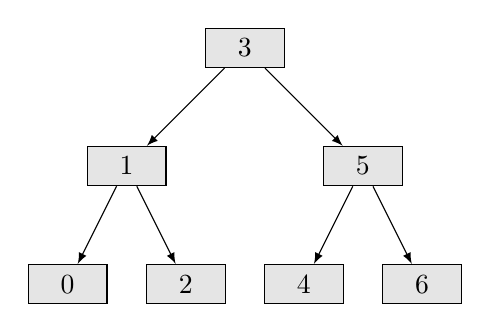
\begin{tikzpicture}
	[
		level distance=1.5cm,
		level 1/.style={sibling distance=3cm},
		level 2/.style={sibling distance=1.5cm},
		edge from parent/.style={draw,-latex}
	]
	\tikzstyle{Node} = [rectangle, minimum width=1cm, minimum height=5mm, text centered, draw=black, fill= gray!20]
	\node [Node]{3}
	child {node [Node]{1}
		child {node [Node]{0}}
		child {node [Node]{2}}
	}
	child {node [Node]{5}
		child {node [Node]{4}}
		child {node [Node]{6}}
	};
\end{tikzpicture}
		
		\caption{Az \texttt{std::set} egy lehetséges ábrázolása, bináris keresőfával. Erre az irányított gráfra igaz, hogy minden gyökér a bal oldali gyerekénél nagyobb, és a jobb oldali gyerekénél kisebb.}\label{fig_std_set}
	\end{figure}
	\subsection{list}
	Az \texttt{std::list} konténer a \texttt{<list>} könyvtár része, és nagyon hasonló ahhoz, mint amit mi írtunk, viszont létezik fejelemmel, és kétirányú.
	\smallskip
	
	Az \texttt{std::vector}-ral szemben ennek a konténernek nincs \texttt{[]} operátora, hiszen mielőtt egy adott indexű elemet vissza tudna adni, el kell oda lépegetnie egyesével. Szögletes zárójel operátort csak akkor szokás írni, hogy ha az nagyon hatékony, lehetőleg konstans műveletigényű, de ez a listánál nem teljesül.
	\begin{note}
		Bár elméletben gyorsabb egy láncolt listába beszúrni a \texttt{vector}-ral (vagy hasonló konténerrel) szemben, hisz csak pár pointert kell átállítani, ez a gyakorlatban csak kivételes esetekben teljesül. Ennek az az oka, hogy bár az elemeket egyesével odébb kell tolni egy vektorban, azok szekvenciálisan vannak a memóriában, és mivel a processzor számít arra, hogy nem csak egy adott elemet, de a környezőket is módosítani szeretnénk, minden alkalommal amikor egy adott elemet kérdezünk le, azzal együtt a környező elemeket is visszaadja nekünk. Ennek következtében kevesebb processzorművelettel végrehajtható a tologatás.
		
		Mivel egy láncolt listában egyesével kell haladni az egyik elemről a következőre, ez gyakran annyira költséges, hogy jobban járunk a vektor alkalmazásával akkor is, ha sokat kell a konténer közepére beszúrni.
		
		Kivételes eset lehet, ha nagyon sok elemből álló listánk van, és azok nagy méretű objektumokat tárolnak, valamint nagyon gyakran kell két elem közé beszúrni. Ilyenkor valóban hatékonyabb tud lenni a \texttt{list}.
	\end{note}
	Mivel már a korábban megismerkedtünk a láncolt listákkal, valamint a korábbi szekciókban mutatott tagfüggvények alkalmazása gyakran teljesen megegyezik a \texttt{list}-nél használatosakkal, túl komoly példákat itt nem fogunk venni. 
	
	Azonban érdemes felhívni a figyelmet egy problémára. Kérdezzük le egy lista harmadik elemét!
	\begin{lstlisting}
#include <iostream>
#include <list>

int main()
{
	std::list<int> l;
	for (int i = 0; i < 5; i++)
		l.push_back(i);
	std::list<int>::iterator it = l.begin();
	++it; ++it;
	std::cout << *it << std::endl; // 2
}
	\end{lstlisting}	
	Az iterátorok léptetésére kell hogy legyen egy egyszerűbb módszer. Írhatnánk egy ciklust, azonban beszédesebb lenne egy léptető függvény írása.
	
	Azonban nem ártana, ha nem csak tetszőleges típust tároló lista iterátorát, hanem tetszőleges konténer iterátorát is tudná ez a függvény léptetni. Mivel az \texttt{std::vector}-nál bármikor ugorhatunk egy tetszőleges elemre, hatékonyabb lenne annak konstans műveletigényű léptető függvényt írni: jó lenne egy olyan algoritmust találni, mely e kettőt egybefoglalja (erre később látunk is majd példát az STL algoritmusoknál).
	
	\medskip
	Ha böngészünk cppreference-en, feltűnhet, hogy az \texttt{std::vector}-ral szemben létezik \texttt{push\_front} és \texttt{pop\_front} metódus: ezeket az \texttt{std::vector}-ral ellentétben konstans idő alatt el lehet végezni (elegendő a fejelemet a rákövetkező elemre állítani és kész is).
	\medskip
	
	Léteznek kifejezetten a listára specifikus műveletek is. Ezek azért nagyon fontosak, mert nem igénylik azt, hogy az adott objektumot lehessen másolni (vagy mozgatni, C++11 szerint). Ez olyankor is fontos lehet, ha például a tárolt objektumok mérete nagyon nagy, és költséges lenne másolni. Példaképp, a \texttt{splice} tagfüggvény egy másik listát (is) vár paraméterül, és azt a listát fűzi be a saját elemei közé.
\begin{lstlisting}
std::ostream& operator<<(std::ostream& out, const std::list<int> &l)
{
	for (std::list<int>::const_iterator it = l.begin(); it != l.end(); it++)
	out << *it << ' ';
	return out;
}	

int main()
{
	std::list<int> list1, list2{};
	for(int i = 0; i<5; i++)
		list1.push_back(i); 
	for(int i = 0; i<5; i++)
		list2.push_front(i);
	std::cout << list1 << std::endl; // 0 1 2 3 4
	std::cout << list2 << std::endl; // 4 3 2 1 0 
	
	list1.splice(list1.end(), list2);
	std::cout << list1 << std::endl; // 0 1 2 3 4 4 3 2 1 0
}
\end{lstlisting}
	Link: \url{http://en.cppreference.com/w/cpp/container/list}
	\subsection{map}
	Az \texttt{std::map} a \texttt{<map>} könyvtárban található. Ez egy egyedi kulcs-érték párokat tároló konténer, mely minden kulcshoz egy értéket rendel. Működése nagyon hasonlít az \texttt{std::set}-ére, annyi különbséggel, hogy párokat tárol (így két kötelező template paramétere van), és mindig a kulcs szerint rendez.
	\smallskip
	
	\begin{figure}[t]
		\centering
		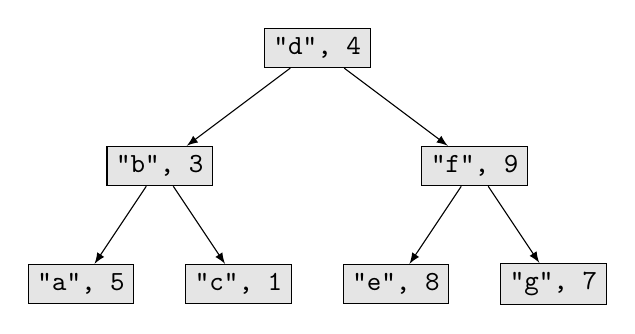
\begin{tikzpicture}
	[
		level distance=1.5cm,
		level 1/.style={sibling distance=4cm},
		level 2/.style={sibling distance=2cm},
		edge from parent/.style={draw,-latex}
	]
	
	\tikzstyle{Node} = [
		rectangle, 
		minimum width=1cm, 
		minimum height=5mm, 
		text centered, 
		draw=black, 
		fill= gray!20
	]
	
	\node [Node]{\texttt{"d", 4}}
	child {node [Node]{\texttt{"b", 3}}
		child {node [Node]{\texttt{"a", 5}}}
		child {node [Node]{\texttt{"c", 1}}}
	}
	child {node [Node]{\texttt{"f", 9}}
		child {node [Node]{\texttt{"e", 8}}}
		child {node [Node]{\texttt{"g", 7}}}
	};
\end{tikzpicture}
		
		\caption{Az \texttt{std::map} egy lehetséges ábrázolása, bináris keresőfával. Az ábrán egy \texttt{std::string, int} párosokat tároló \texttt{map} szerepel -- figyeljük meg, hogy a a konténer a kulcs szerint rendez, az értékek a rendezés szempontjából nem számítanak.}\label{fig_std_map}
	\end{figure}
	Van egy speciális beszúró függvénye is:
\begin{lstlisting}
#include <map>
#include <iostream>

int main()
{
	std::map<std::string, int> m;
	m["Hello"] = 42;
	m["xyz"] = 8;
	m["Hello"] = 9;
	std::cout << m.size() << std::endl; // 2
	std::cout << m["Hello"] << std::endl; // 9
}
\end{lstlisting}
	A \texttt{[]} operátor egy új kulcsot hoz létre, és ahhoz rendel egy új értéket. Az utolsó sornál mivel a \texttt{''Hello''}-t már tartalmazza a map, így annak az értékét felülírja.
	
	\medskip
	Sajnos ez az operátor azonban okozhat pár kellemetlen meglepetést is.
	\begin{lstlisting}
int main()
{
	std::map<std::string, int> m;
	std::cout << m.size() << std::endl; // 0
	if(m["c++"] != 0)
		std::cout << "nem 0" << std::endl;
	std::cout << m.size() << std::endl; // 1
}
	\end{lstlisting}
	A \texttt{[]} operátor úgy működik, hogy ha a \texttt{map} nem tartalmazza a paraméterként kapott kulcsot, akkor létrehozza és beszúrja, ha benne van, visszaadja az értékét. Bár mi nem tettük bele azt hogy \texttt{c++} szándékosan, de pusztán azzal, hogy rákérdeztünk, akaratlanul is megtettük. (Figyeljük meg, hogy akkor tudnánk új elemet hozzátenni, ha azt írnánk pl. hogy \texttt{m["C++"] = 3}; azonban mi nem adtunk meg ehhez a kulcshoz értéket. Ilyenkor a map alapértelmezett értéket rendel a kulcshoz, szám típusoknál 0-t, így be fog szúrni egy \texttt{("c++", 0)} párt.)
	\begin{lstlisting}
bool contains(const std::map<std::string, int> &m)
{
	//m["c++"]; fordítási hiba: [] operator nem konstans függvény.
	return m.find("C++") != m.end();
}
	\end{lstlisting}
	Ez a függvény helyesen vizsgálja, hogy a \texttt{c++} benne van-e. (Ha cppreference-en rákeresünk, a \texttt{map}-nek a \texttt{find} nevű tagfüggvénye egy iterátort ad vissza a talált elemre, illetve visszaadja egy past-the-end iterátort ha nem találja meg.)
	\medskip
	
	
	\texttt{std::map}-ban az iterálás kicsit trükkösebb, ugyanis \texttt{std::map} párokat tárol, méghozzá egy más alapból megírt struktúrát használ, az \texttt{std::pair}-t, ami kb. így néz ki:
	\begin{lstlisting}
template <typename T1, typename T2>
struct pair
{
	T1 first;
	T2 second;
};
	\end{lstlisting}
	Így az az adott kulcs ill. érték lekérdezése így fog kinézni:
	\begin{lstlisting}
for(std::map<std::string, int>::iterator i = m.begin(); i != m.end(); i++)
{
	std::cout << i->first << " " << i->second;
}
	\end{lstlisting}
	Amennyiben új elemeket szúrunk be, gyakran megkerülhető a problémás \texttt{[]} használata. Az \texttt{std::map} insert függvénye egy \texttt{std::pair}-t vár paraméterül, melyet könnyen tudunk alkotni \texttt{std::make\_pair} függvény segítségével.
	\begin{lstlisting}
std::map<int, char> m;
m.insert(std::make_pair(1, 'a'));
	\end{lstlisting}
	
	Link: \url{http://en.cppreference.com/w/cpp/container/map}
	\begin{note}
		Az \texttt{std::multimap} ehhez szintén hasonló, így gyakorlásként ezt ismét az olvasóra bíznám.
	\end{note}
\end{document}
